\documentclass[aspectratio=1610, handout]{beamer}
\usepackage[utf8]{inputenc}
\usepackage{ragged2e}
\usepackage{xcolor}
\usepackage[italian]{babel}
\usepackage{multirow}
\usetheme[progressbar=frametitle,titleformat=smallcaps]{metropolis}
\setbeamertemplate{frame numbering}[fraction]
\setbeamercovered{dynamic}
\definecolor{rosso}{RGB}{255, 0, 0}
\definecolor{giallo}{RGB}{254,212,23}
\hypersetup{colorlinks=true,linkcolor=black,urlcolor=rosso}
\setbeamercolor{palette primary}{fg=black, bg=giallo}
\setbeamercolor{background canvas}{bg=white}
\setbeamercolor{normal text}{fg=black}
\setbeamercolor{progress bar}{fg=rosso}
\setbeamercolor{framesubtitle}{fg=rosso}
\setbeamercolor{normal text .dimmed}{fg=giallo}
\setbeamercolor{block title alerted}{fg=rosso, bg=giallo}
\setbeamerfont{caption}{size=\tiny}
\setbeamerfont{caption name}{size=\tiny}
\setlength{\abovecaptionskip}{0pt}
\makeatletter
\metroset{block=fill}
\setlength{\metropolis@progressinheadfoot@linewidth}{1pt} 
\setlength{\metropolis@progressonsectionpage@linewidth}{1pt}
\setlength{\metropolis@titleseparator@linewidth}{1pt}
\makeatother

\title{PROTOCOLLI DI RETE}
\subtitle{HTTP, IP, DHCP, DNS}
\date{}
\institute{\textit{
        Fonti:
        \begin{itemize}
            \item[-] \href{https://it.wikipedia.org/wiki/Protocollo_di_rete}{Wikipedia}
            \item[-] \href{https://www.forbes.com/advisor/it/business/software/ipv6-protocollo-vpn/}{Forbes}
        \end{itemize}
    }
}

\begin{document}

\begin{frame}[plain, noframenumbering]
    \titlepage
\end{frame}

\section{DEFINIZIONE}

\begin{frame}{PROTOCOLLO DI RETE}
    \begin{alertblock}{DEFINIZIONE}
        \begin{minipage}{0.98\linewidth}
            \justifying
            Un protocollo di comunicazione, è un \textbf{insieme di regole} formalmente descritte 
            che definiscono le modalità di comunicazione tra due o più entità. Ogni protocollo 
            è progettato con precisi compiti e finalità, a seconda delle entità interessate e 
            del mezzo di comunicazione. Se le due entità sono remote, si parla di \textbf{protocollo di rete}.\\
            \bigskip
            \tiny{\textbf{Curiosità}}\\
            \tiny{\href{https://www.w3.org/}{Chi gestisce gli standard per i protocolli?}}           
        \end{minipage}
    \end{alertblock}
\end{frame}

\section{HTTP (Hypertext Transfer Protocol)}

\begin{frame}{HTTP}
    \begin{alertblock}{DEFINIZIONE}
        \begin{minipage}{0.98\linewidth}
            \justifying
            l'HyperText Transfer Protocol (\textbf{HTTP}) è un protocollo a livello applicativo 
            usato come principale sistema per la \textbf{trasmissione d'informazioni sul web}. La prima 
            versione dell'HTTP, risale alla fine degli anni '80 e tutt'ora costituisce, insieme al 
            linguaggio HTML e gli \textbf{URL} (Uniform Resource Locator), il nucleo base 
            del \textbf{WWW} (World Wide Web).\\
            \bigskip
            \tiny{\textbf{Curiosità}}\\
            \tiny{\href{https://www.w3.org/}{Chi gestisce gli standard per i protocolli?}}           
        \end{minipage}
    \end{alertblock}
\end{frame}

\begin{frame}{HTTP GET}
    \only<1| handout:1>{\begin{figure}
        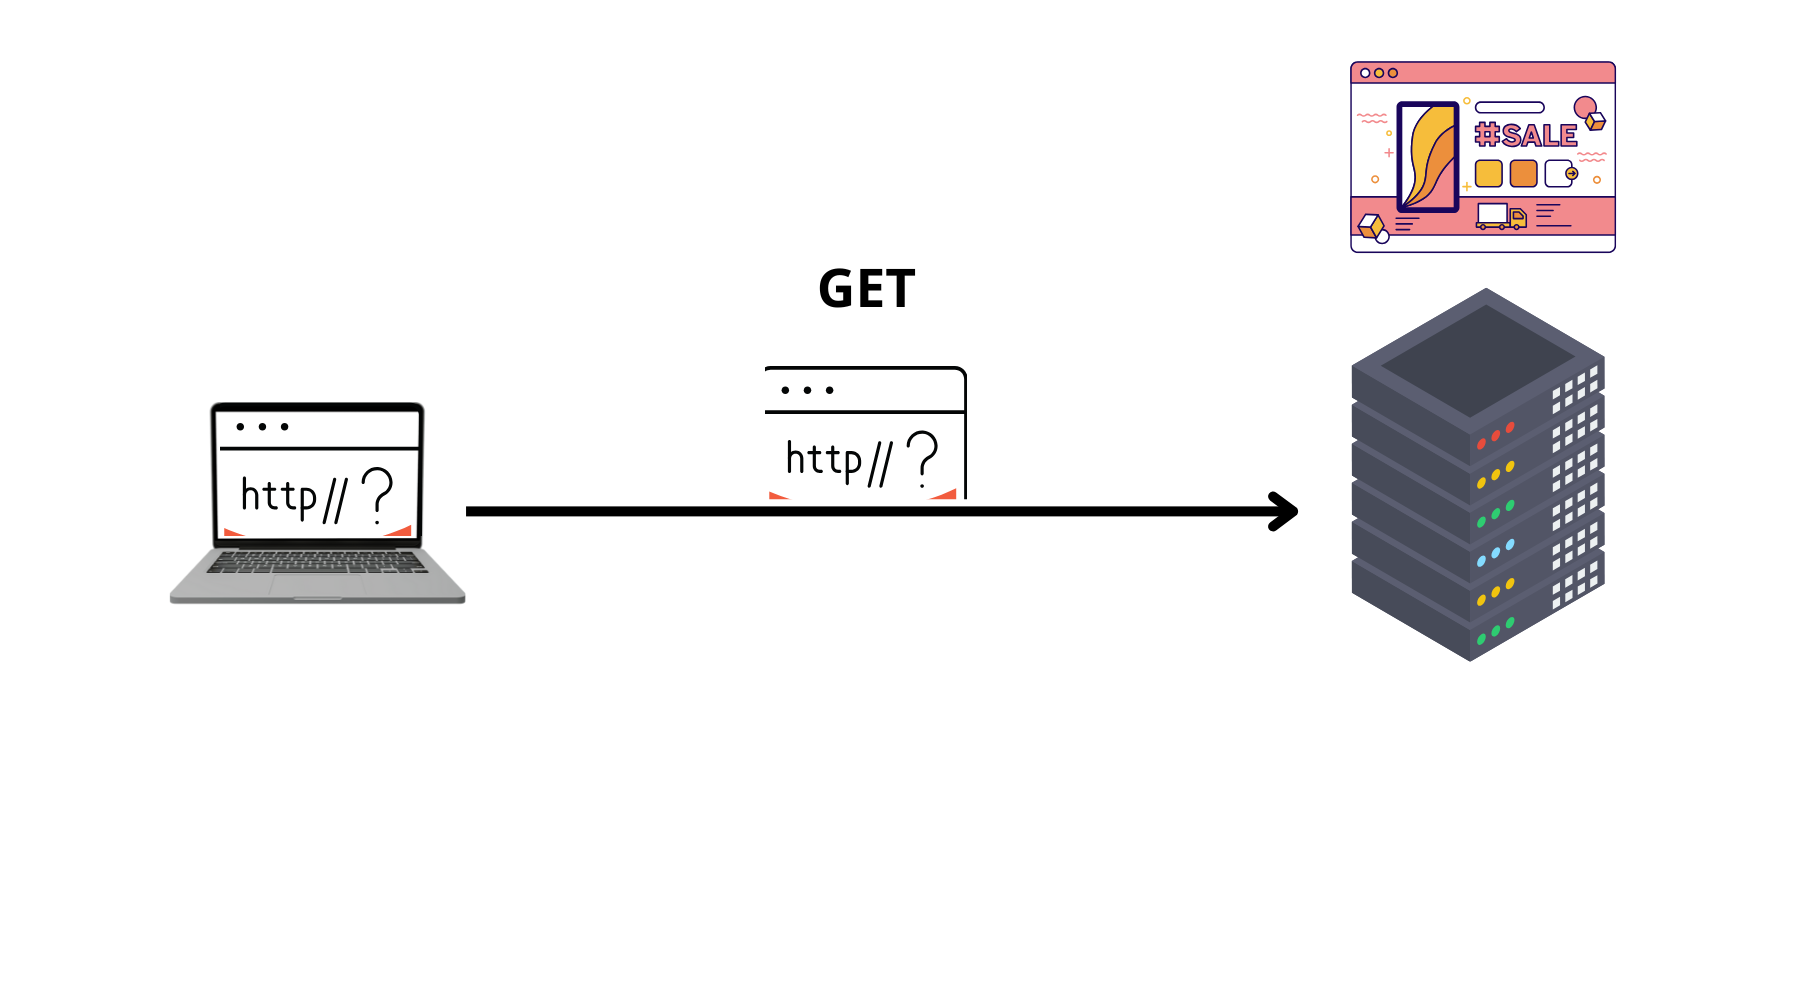
\includegraphics[width=\linewidth]{img/httpGET4.png}
        \caption{{creata con \href{https://www.canva.com/}{Canva}}}
    \end{figure}}
    \only<2| handout:2>{\begin{figure}
        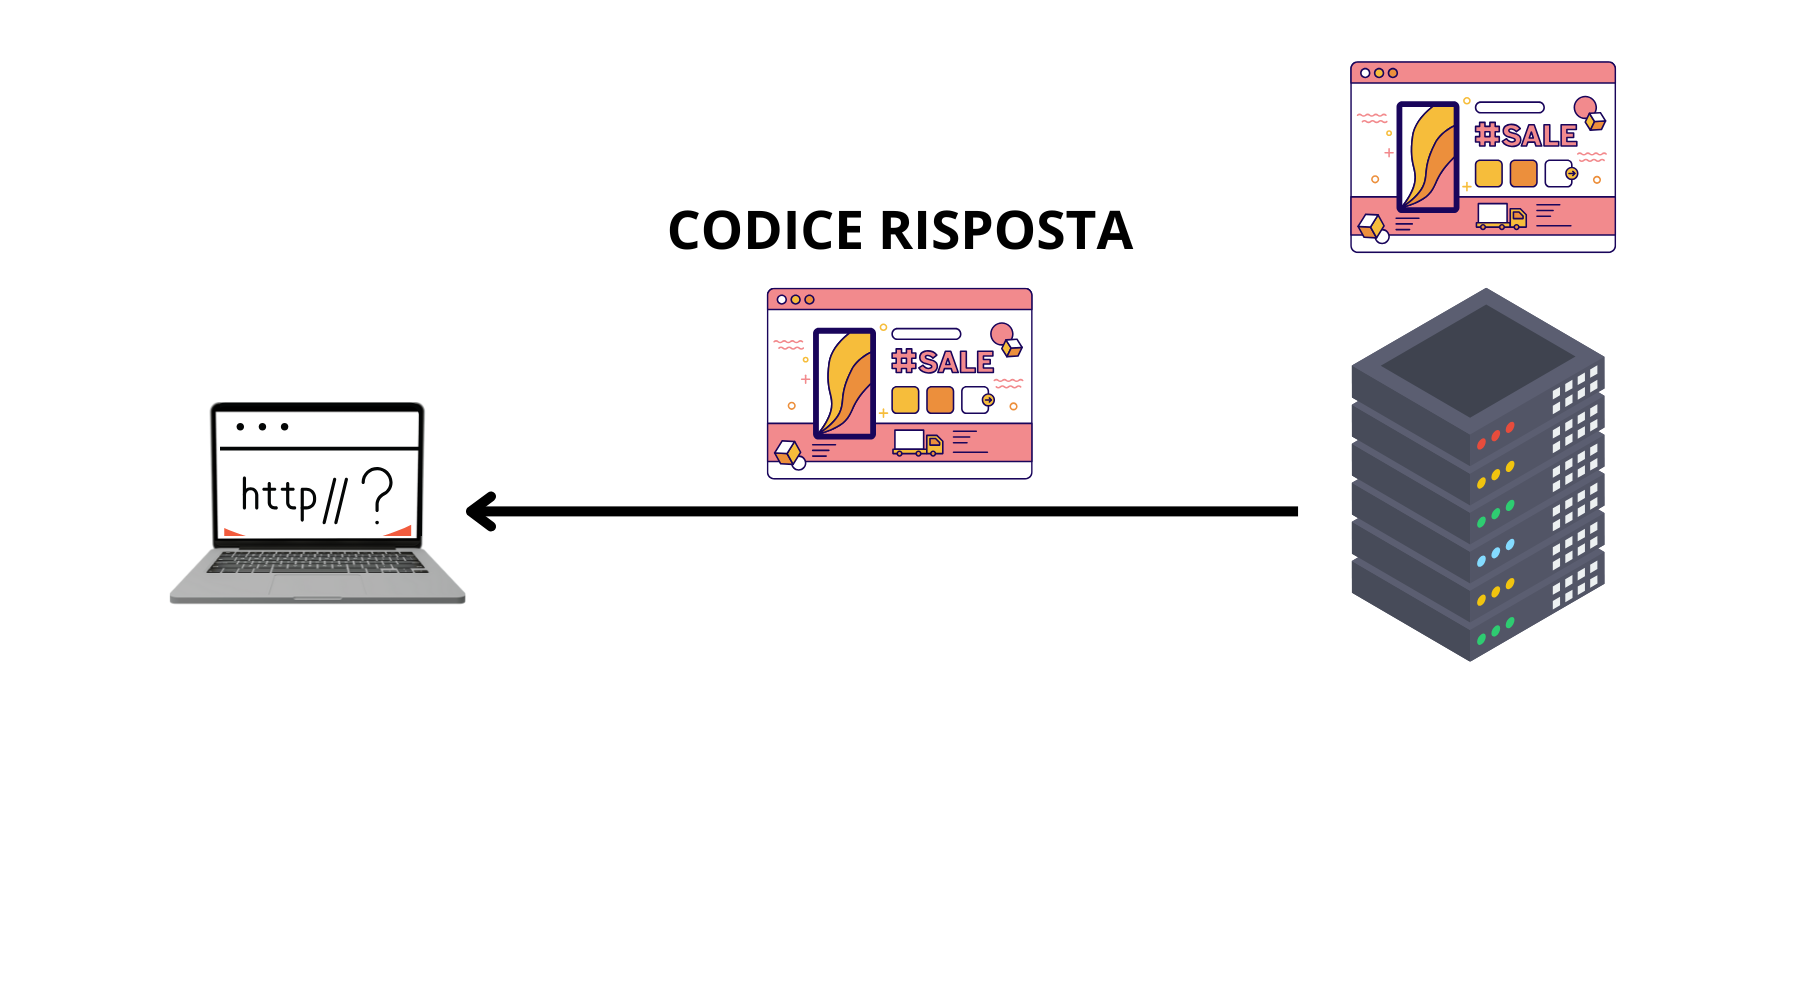
\includegraphics[width=\linewidth]{img/httpGET5.png}
        \caption{{creata con \href{https://www.canva.com/}{Canva}}}
    \end{figure}}
    \only<3| handout:3>{\begin{figure}
        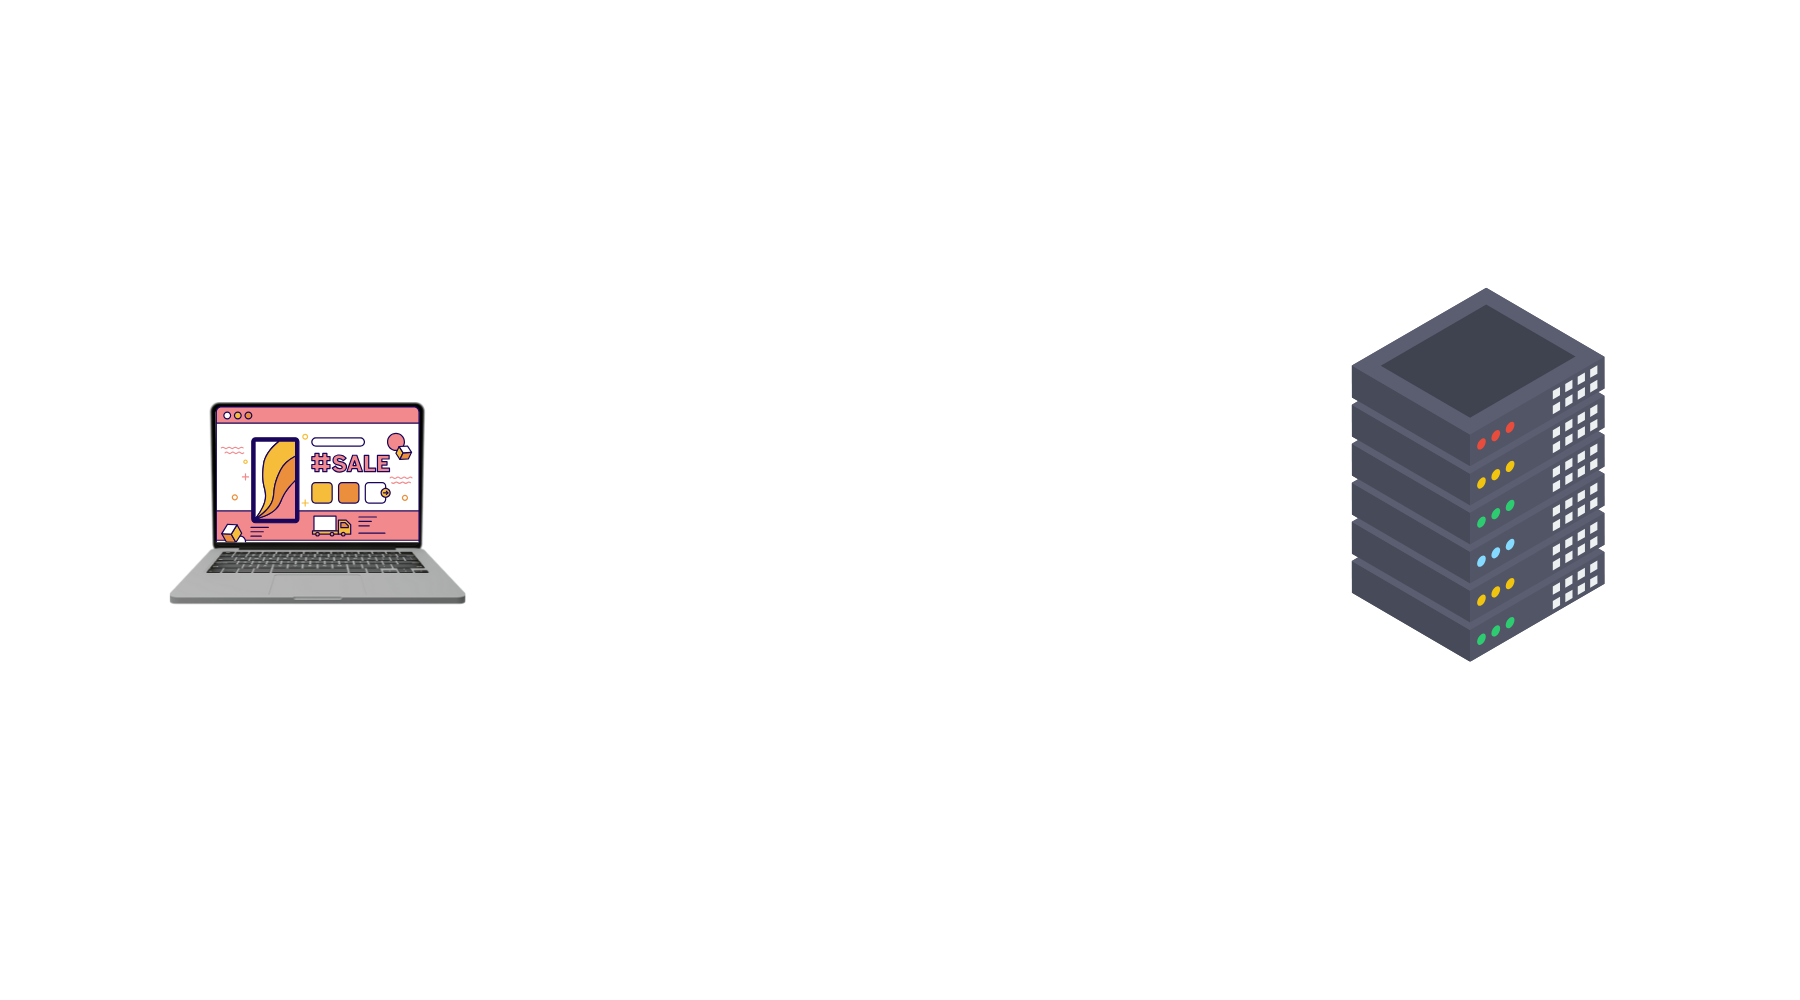
\includegraphics[width=\linewidth]{img/httpGET6.png}
        \caption{{creata con \href{https://www.canva.com/}{Canva}}}
    \end{figure}}
\end{frame}

\begin{frame}{CODICI DI RISPOSTA}
    \centering
    \begin{tabular}{c||l}
        \textbf{CODICE} & \textbf{DESCRIZIONE} \\
        \hline
        \hline
        \pause
        200 OK & Il server ha fornito correttamente il contenuto.\\
        \hline
        \pause
        404 Not Found & La risorsa richiesta non è stata trovata.\\
        \hline
        \pause
        \multirow{2}*{500 Internal Server Error} & \multirow{2}{8cm}{Il server non è in grado di rispondere alla richiesta per un suo problema interno.}\\
        \\
        \hline
    \end{tabular}
\end{frame}

\section{IP (Internet Protocol)}

\begin{frame}{IP}
    \begin{alertblock}{DEFINIZIONE}
        \begin{minipage}{0.98\linewidth}
            \justifying
            L’Internet Protocol è il protocollo di rete \textbf{responsabile dell'indirizzamento e instradamento} 
            dei pacchetti di dati da una sorgente (identificata da un indirizzo IP) ad una 
            destinazione (identificata da un altro indirizzo IP). Un \textbf{indirizzo IP} è un numero che \textbf{identifica univocamente} 
            ogni dispositivo appartenente ad una rete informatica. Ne esistono due versioni:
            \begin{itemize}
                \pause
                \item \textbf{IPv4}: formato da 32 bit suddivisi in 4 gruppi da 8 bit. Nella notazione decimale è 
                rappresentato da 4 numeri compresi tra 0 e 255 separati da un punto. Esempio: \textbf{192.168.0.1}
                \pause
                \item \textbf{IPv6}: formato da 128 bit suddivisi in 8 gruppi da 16 bit. Nella notazione esadecimale è 
                rappresentato da 8 numeri compresi tra 0000 e ffff separati dal carattere ":". Esempio: \textbf{2001:0bd8:85a3:0000:0000:8e2a:0370:7334}
            \end{itemize}
            \bigskip
            \tiny{\textbf{Curiosità}}\\
            \tiny{\href{https://it.wikipedia.org/wiki/Saturazione_di_IPv4}{Perchè ne esistono due versioni?}}            
        \end{minipage}
    \end{alertblock}
\end{frame}

\begin{frame}{INDIRIZZI IP PUBBLICI VS PRIVATI}
    \centering
    \begin{tabular}{c||c||c}
        & \textbf{IP PUBBLICO} & \textbf{IP PRIVATO} \\
        \hline
        \hline
        \pause
        \multirow{2}{2,5cm}{\textbf{DEFINIZIONE}} & \multirow{2}{5cm}{Viene assegnato dal fornitore di servizio (\href{https://www.facile.it/adsl/compagnie.html}{ISP})} & \multirow{2}{5cm}{Utilizzato all'interno delle reti locali LAN} \\
        & & \\
        \hline
        \pause
        \multirow{2}{2,5cm}{\textbf{SCOPO}} & \multirow{2}{5cm}{Indentifica un dispositivo nella rete Internet} & \multirow{2}{5cm}{Identifica un dispositivo in una rete locale} \\
        & & \\
        \hline
        \pause
        \multirow{2}{2,5cm}{\textbf{VISIBILIT\'A}} & \multirow{2}{5cm}{Accessibile da qualsiasi dispositivo connesso a Internet} & \multirow{2}{5cm}{Non accessibile direttamente dall'esterno della rete locale} \\
        & & \\
        \hline
        \pause
        \multirow{2}{2,5cm}{\textbf{UTILIZZO}} & \multirow{2}{5cm}{Server Web, router, servizi pubblici (pagine web, ecc.)} & \multirow{2}{5cm}{Dispositivi domestici (pc, smartphone, ecc.), reti LAN} \\
        & & \\
        \hline
    \end{tabular}
\end{frame}

\begin{frame}{INDIRIZZI IP STATICI VS DINAMICI}
    \centering
    \begin{tabular}{c||c||c}
        & \textbf{IP STATICO} & \textbf{IP DINAMICO} \\
        \hline
        \hline
        \pause
        \multirow{2}{2,5cm}{\textbf{DEFINIZIONE}} & \multirow{2}{5cm}{Assegnato manualmente a un dispositivo/Assegnato dall'ISP} & \multirow{2}{5cm}{Assegnato automaticamente a un dispositivo tramite \textbf{DHCP}} \\
        & & \\
        \hline
        \pause
        \multirow{2}{2,5cm}{\textbf{PROPRIET\'A}} & \multirow{2}{5cm}{Non cambia nemmeno dopo il riavvio del dispositivo} & \multirow{2}{5cm}{Cambia periodicamente o dopo il riavvio del dispositivo} \\
        & & \\
        \hline
        \pause
        \multirow{3}{2,5cm}{\textbf{VANTAGGI}} & \multirow{3}{5cm}{Connessioni stabili per servizi che richiedono raggiungibilità continua} & \multirow{3}{5cm}{Non richiede configurazione manuale, gestito dal protocollo DHCP} \\
        & & \\
        & & \\
        \hline
        \pause
        \multirow{3}{2,5cm}{\textbf{SVANTAGGI}} & \multirow{3}{5cm}{Potrebbe esporre maggiormente a rischi di sicurezza} & \multirow{3}{5cm}{Può cambiare nel tempo, meno adatto a servizi che richiedono stabilità di connessione} \\
        & & \\
        & & \\
        \hline
    \end{tabular}
\end{frame}

\section{DHCP (Dynamic Host Configuration Protocol)}

\begin{frame}{DHCP}
    \begin{alertblock}{DEFINIZIONE}
        \begin{minipage}{0.98\linewidth}
            \justifying
            Il \textbf{DHCP} è un protocollo di rete che \textbf{automatizza l'assegnazione degli indirizzi IP} ai 
            dispositivi di una rete.\\
            \bigskip
            Esempio nella LAN domestica:            
            \begin{enumerate}
                \pause
                \item Un \textbf{dispositivo} (client) che si connette alla rete \textbf{invia una richiesta DHCP} al modem;
                \pause
                \item Il modem (server DHCP) risponde con il \textbf{primo indirizzo IP privato dinamico disponibile};
                \pause
                \item  Il dispositivo (client) \textbf{utilizza l'indirizzo IP} per un periodo limitato e \textbf{lo rilascia
                quando si scollega} dalla rete.
            \end{enumerate}            
            Il protocollo quindi automatizza la configurazione di rete, riducendo errori e semplificando la 
            gestione di reti con molti dispositivi.
        \end{minipage}
    \end{alertblock}
\end{frame}

\section{DNS (Domain Name System)}

\begin{frame}{DNS}
    \begin{alertblock}{DEFINIZIONE}
        \begin{minipage}{0.98\linewidth}
            \justifying
            Il DNS è un protocollo di rete utilizzato per \textbf{assegnare nomi testuali ai 
            nodi della rete}. L'operazione di conversione da nome a indirizzo IP è detta 
            "\textbf{risoluzione DNS}"; la conversione da indirizzo IP a nome testuale è detta "\textbf{risoluzione 
            inversa}". I nomi testuali sono utilizzabili al posto degli indirizzi IP originali per 
            \textbf{facilitare la navigazione in rete da parte dell'utente}.\\
            \bigskip
            Esempio di risoluzione inversa:
            \begin{enumerate}
                \pause
                \item Copia l'URL del sito della scuola;
                \pause
                \item Inserisci l'URL nel sito: \href{https://www.nslookup.io/}{nslookup} per effettuare la risoluzione inversa;
                \pause
                \item Analizza le informazioni che si possono ottenere. 
            \end{enumerate}
            \bigskip
            \tiny{\textbf{Curiosità}}\\
            \tiny{\href{https://adguard-dns.io/it/welcome.html}{Utilizzare il DNS per aumentare la propria privacy}}            
        \end{minipage}
    \end{alertblock}
\end{frame}

\end{document}